
\documentclass{sig-alternate-05-2015}
\usepackage{placeins}
\usepackage{hyperref}


\begin{document}

\title{WolfPlanner: Personalized Task Scheduling Bot}

\numberofauthors{4} 
\author{
% You can go ahead and credit any number of authors here,
% e.g. one 'row of three' or two rows (consisting of one row of three
% and a second row of one, two or three).
%
% The command \alignauthor (no curly braces needed) should
% precede each author name, affiliation/snail-mail address and
% e-mail address. Additionally, tag each line of
% affiliation/address with \affaddr, and tag the
% e-mail address with \email.
%
% 1st. author
\alignauthor
Neel Kapadia\\
       \affaddr{North Carolina State University}\\
       \affaddr{Raleigh, NC, US}\\
       \email{ntkapadi@ncsu.edu}
% 2nd. author
\alignauthor
Rohan Chandavarkar\\
       \affaddr{North Carolina State University}\\
       \affaddr{Raleigh, NC, US}\\
       \email{rgchanda@ncsu.edu}
% 3rd. author
\alignauthor 
Sainag Shetty\\
       \affaddr{North Carolina State University}\\
       \affaddr{Raleigh, NC, US}\\
       \email{sgshetty@ncsu.edu}
\and  % use '\and' if you need 'another row' of author names
% 4th. author
\alignauthor 
Rohit Naik\\
       \affaddr{North Carolina State University}\\
       \affaddr{Raleigh, NC, US}\\
       \email{rtnaik@ncsu.edu}
}
\date{01 Feb 2018}
% Just remember to make sure that the TOTAL number of authors
% is the number that will appear on the first page PLUS the
% number that will appear in the \additionalauthors section.

\maketitle
\begin{abstract}
With the number of tasks increasing day-by-day, it is becoming difficult for individuals to manage so many tasks considering the varying amount of time available and required to complete them. It requires continuous and active effort to create weekly/bi-weekly schedules. This leads to wastage of valuable time, and poor planning might lead to excessive workloads. In such situations, an application that makes a schedule (time-table) for the individuals taking into account their deadlines and dependencies between tasks will be a great asset. 
\par
In this paper, we intend to develop an application which will generate a schedule for users based on their upcoming tasks such as assignments, projects, interviews, other events, etc (information about which will be given to the system by them). On conduting a user survey, we found that many users face an issue in scheduling team meetings. Hemce, we plan to develop an algorithm which will match the availability of the team and suggest possible timings to schedule the meeting. Furthermore, to keep up with the current technology trend of interactive assistants, we plan to integrate this service with a Slack chatbot thereby avoiding downloading of a stand-alone application. For now, we restrict our domain of users to university students for ease of data collection and implementation.
\end{abstract}


%
% The code below should be generated by the tool at
% http://dl.acm.org/ccs.cfm
% Please copy and paste the code instead of the example below. 
%




%
% End generated code
%

%
%  Use this command to print the description
%
\printccsdesc

% We no longer use \terms command
%\terms{Theory}

\keywords{Scheduler, Chatbot, Calendar, Meeting, Time-table, Planner}

\section{Introduction}
\par
In this paper, we propose a personalized time management bot for students.
\par
Students need to focus on important tasks such as their coursework and studies and leave the lesser menial tasks such as making daily time-tables to be automated for them. Today, it is a world of personal interactive assistants and according to Gartner\'s report\cite{planner1}, 85\% of customer interactions will be managed without a human by 2020. So we propose to develop a chatbot that is able to assist the user in scheduling a wide range of day-to-day tasks which may include classes, assignments, project meetings, discussions and readings to name a few. The application we are proposing is a chatbot interface which will take in all of this information as input from students to help them manage their time efficiently. 
\par
Also, in universities, students are involved in many group activities, and scheduling these meet-ups are often challenging due to conflicting schedules. They take up a lot of time and lead to hassles. So, having a collaborative approach is needed. The bot we propose, will automate this scheduling conundrum by suggesting meeting times based on common availability of the team. To maintain the privacy of the users' time, the system will suggest schedules only if all the members of the group have provided permission to the system to read their schedule.
\par
The motive of our work is to develop a Chatbot with which a user can communicate, provide data, ask for change in schedule, etc. The bot generates schedules on a weekly or biweekly basis as per user preference. The user requests a set of tasks every week and also sets the priority to each of them. As per the user preference, the bot will generate an appropriate schedule taking into account all of the details. Further, this generated schedule may be exported to Google Calendar for easy access across all the devices.
\par
We will host our system on Amazon Web Services and the user data will be stored on MongoDB. Amazon Web Services will provide scalability and reliability  to our system, and security to users' data. The user details will be stored as objects on the NoSQL MongoDB environment making it convenient to access the details of the user who is logged in without any  requirement of costly join operations which would have been needed in case of relational databases. Also storing user data in tables might lead to redundancy and lot of NULL data. Hence, we decided to use MongoDB as our database system.
\par
To provide a gist of what the bot does:
\begin{itemize}
\par
  \item Accept information about classes, assignments, projects, etc. from the user
  \item Generate a schedule for the user based on input
  \item Organize project meetings based on availability of all members
  \item Give the Student the option to add the generated schedule to Google calendar
\end{itemize}
\begin{figure}
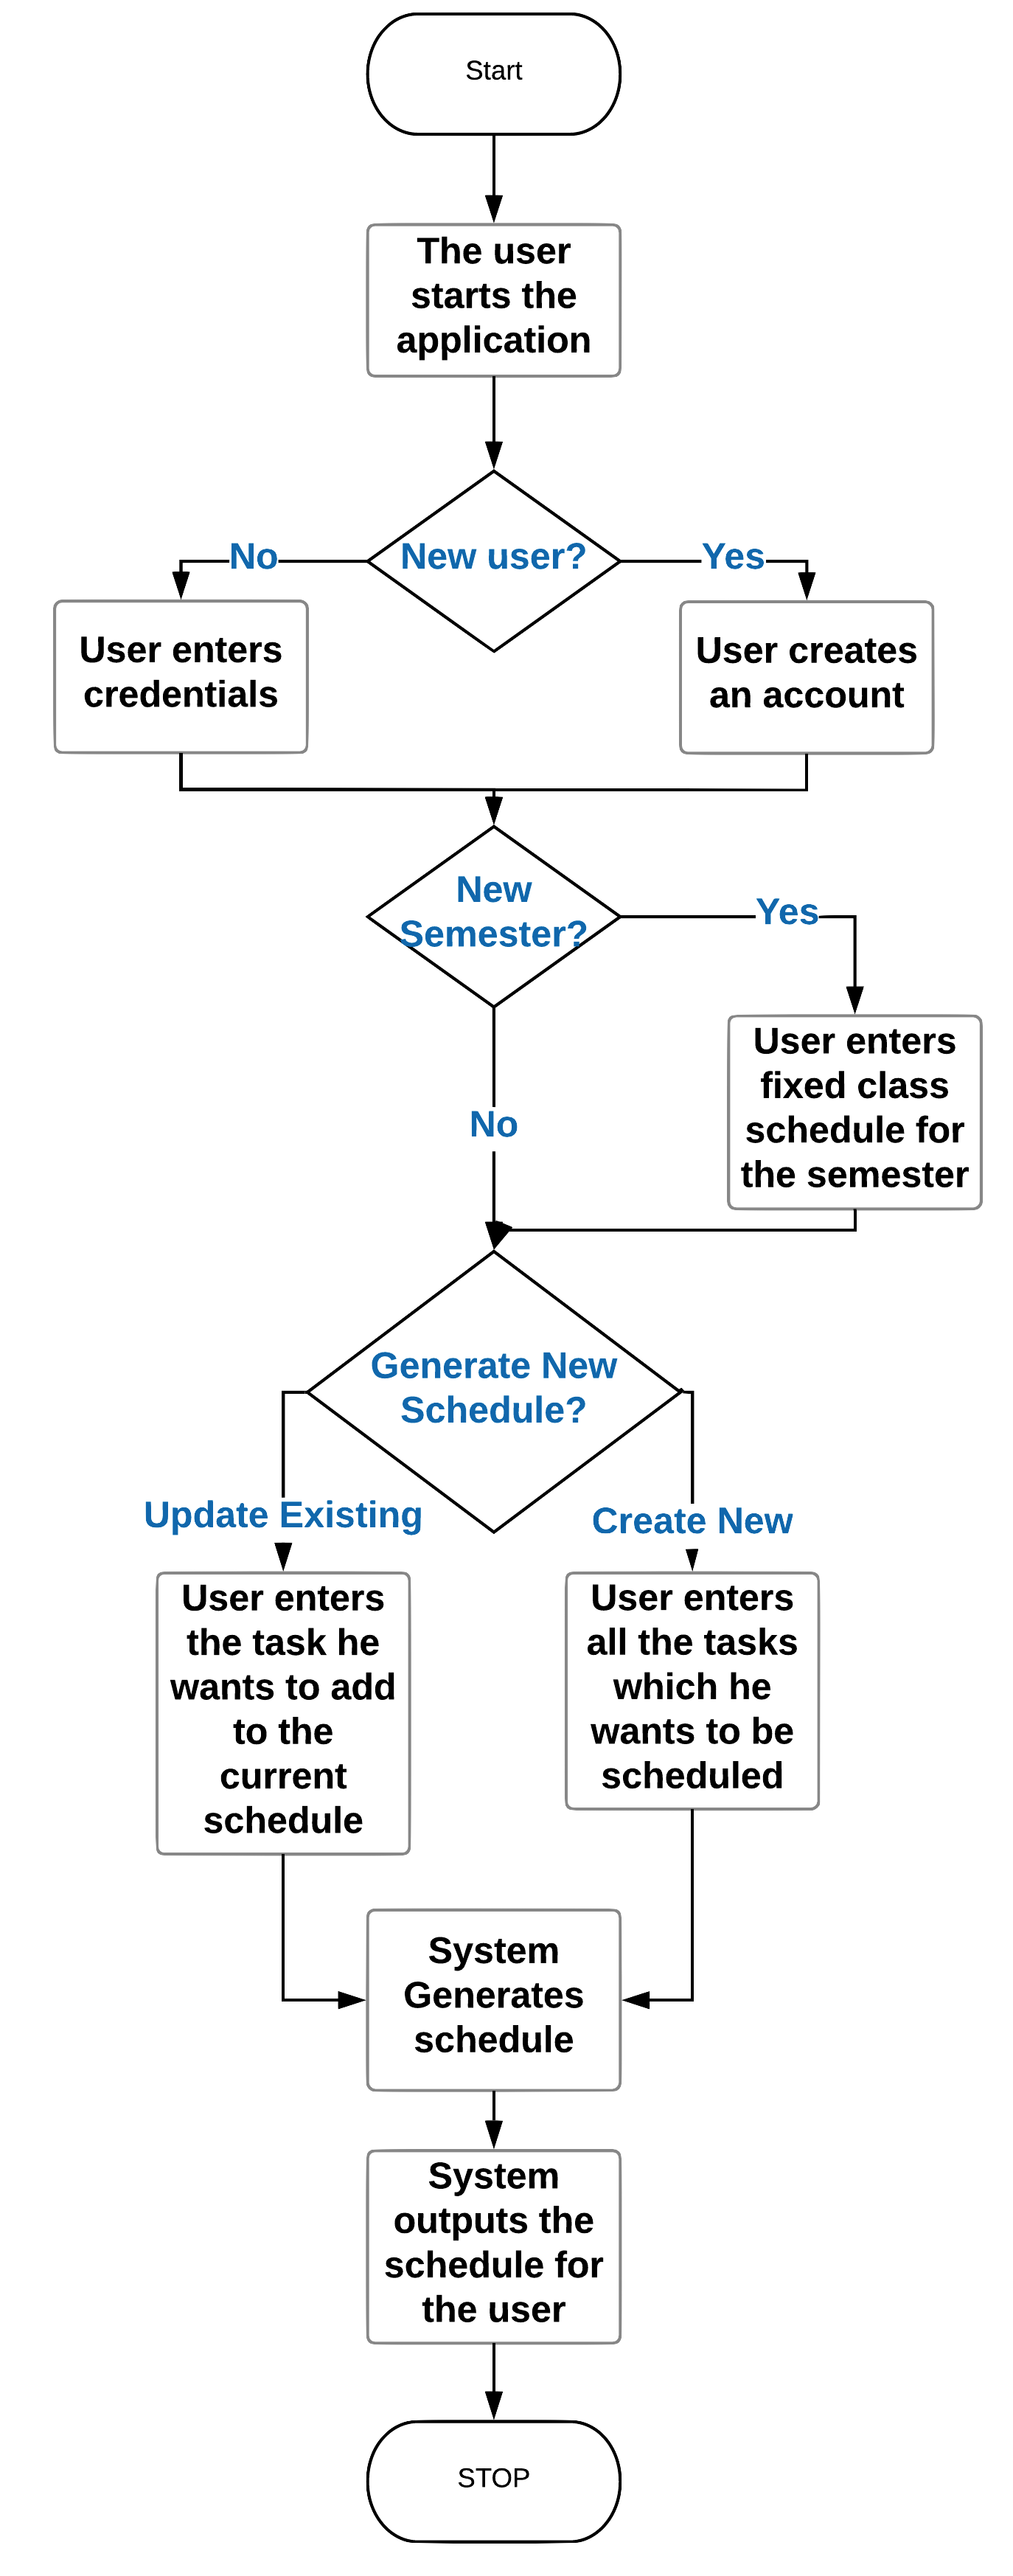
\includegraphics[scale = 0.36]{ActivityDiagram}
\centering
\caption{Activity Diagram}
\end{figure}

\section{Motivation}
A major problem in students life is managing homeworks, projects, interviews, meetings etc. and still get some free time. Our study revealed that majority of survey respondents (77\%) want an application/bot which generates a schedule for them. However, a lot of people (74\%) don't use any calendar for organizing their day. This shows us that people want an application for a functionality (generating a time-table with time-wise task distributions) which other calendars don't provide. Hence, we came up with this idea to fulfill the users' requirement, by creating an interactive bot which generates schedules (time-tables) for the user and also organizes meeting times for them. This will help the users manage their time efficiently and work productively.



\section{Literature Review}
Despite the success of calender tools in organizing and tracking activities, a lot of time is spent by people on managing their time properly. Berry et al.\cite{planner2} came up with PTime, a personalized time management agent which reduces this problem of time management considerably, when it comes to arranging meetings. PTime schedules meetings based on factors like participants, time and locations. Our bot will go a step further and automatically schedule each and every task of a user along with the meetings.
\par
The biggest challenges in any task planner are the constraints in schedules and which scheduling method is used.
\par
The performance of a scheduling algorithm depends on the following:
\begin{itemize}
  \item Constraints in scheduling
  \item Preemptive tasks
  \item Penalty for errors in scheduling
\end{itemize}
\par
Traditional algorithms face a lot of problems when it comes to preemptive scheduling. For example, schedule quality of FCFS scheduling algorithm is highly sensitive to the preemption strategy used. Schwiegelshohn et al.\cite{planner3} demonstrated that by doing certain improvements in FCFS it can be better than any of the other preemptive algorithms but the parameter settings and efficiency depends heavily on the workload. As our task scheduler deals with multiple tasks which can arrive at any time, using FCFS might lead to compromising efficient task scheduling as our workload itself is dynamic in nature.
\par
After reviewing some papers we came to the conclusion that the algorithm implemented by L. J. Wilkerson et al.\cite{planner4} will be the most effective algorithm for our task scheduler. The authors have assumed that the tasks are independent and simultaneously available for scheduling. The criterion used to judge the efficiency of the scheduling is the total tardiness of the task set. A task contributes to tardiness if it is completed after its due date, otherwise it contributes 0 to the level of tardiness.The decision rule does not strictly follow earliest deadline first or shortest task first strategy, but it is a combination of both. When comparing two tasks, it schedules the task which has the earlier deadline. If the task which has earlier deadline has processing time which contributes to tardiness, that is if it crosses both the deadlines, then the shorter task is executed first.




\section{Use Case}
Our system has just one actor i.e. the User of the system. The User has a variety of use cases, as follows - 
% to fill in a form at the start of every semester to add the fixed tasks over the semester such as classes and assignments. The User can perform various functions like - Add a new task to be included in the schedule, Generate schedule, Make schedule final, Schedule a meeting with other users. If the User is happy with the generated schedule, he has an option of adding the entries to Google Calendar. Otherwise, he can modify the schedule to reflect the changes desired.
\begin{enumerate}
\item Fill form for details - Whenever the user starts a new cycle such as a new semester, he/she will have to fill a form with all the fixed tasks for that cycle.
\item Add new task - This functionality will be present to allow the user to add any tasks such as project group or other meetings, which can change over time due to various unforeseen reasons.
\item Generate schedule - When the user is ready after filling in the tasks, he/she can generate the schedule for the week.
\item Add to calendar - If the user is happy with the generated schedule, he/she would get an option to add all the events to Google Calendar.
\item Modify schedule - If the user is not completely happy with the generated schedule, he/she can modify that portion of the schedule he/she is not happy with.
\item Check user availability - This functionality will allow the user to request other users to share their availability, for setting up a meeting with them. After the other users approve this request, a common free time between the users will be displayed.
\item Schedule a meeting - With this functionality, the user can decide which of the common available time slots obtained from the 'Check user availability' use case is the best for the meeting and will then finalize the meeting.
\end{enumerate}
\begin{figure}[!htbp]
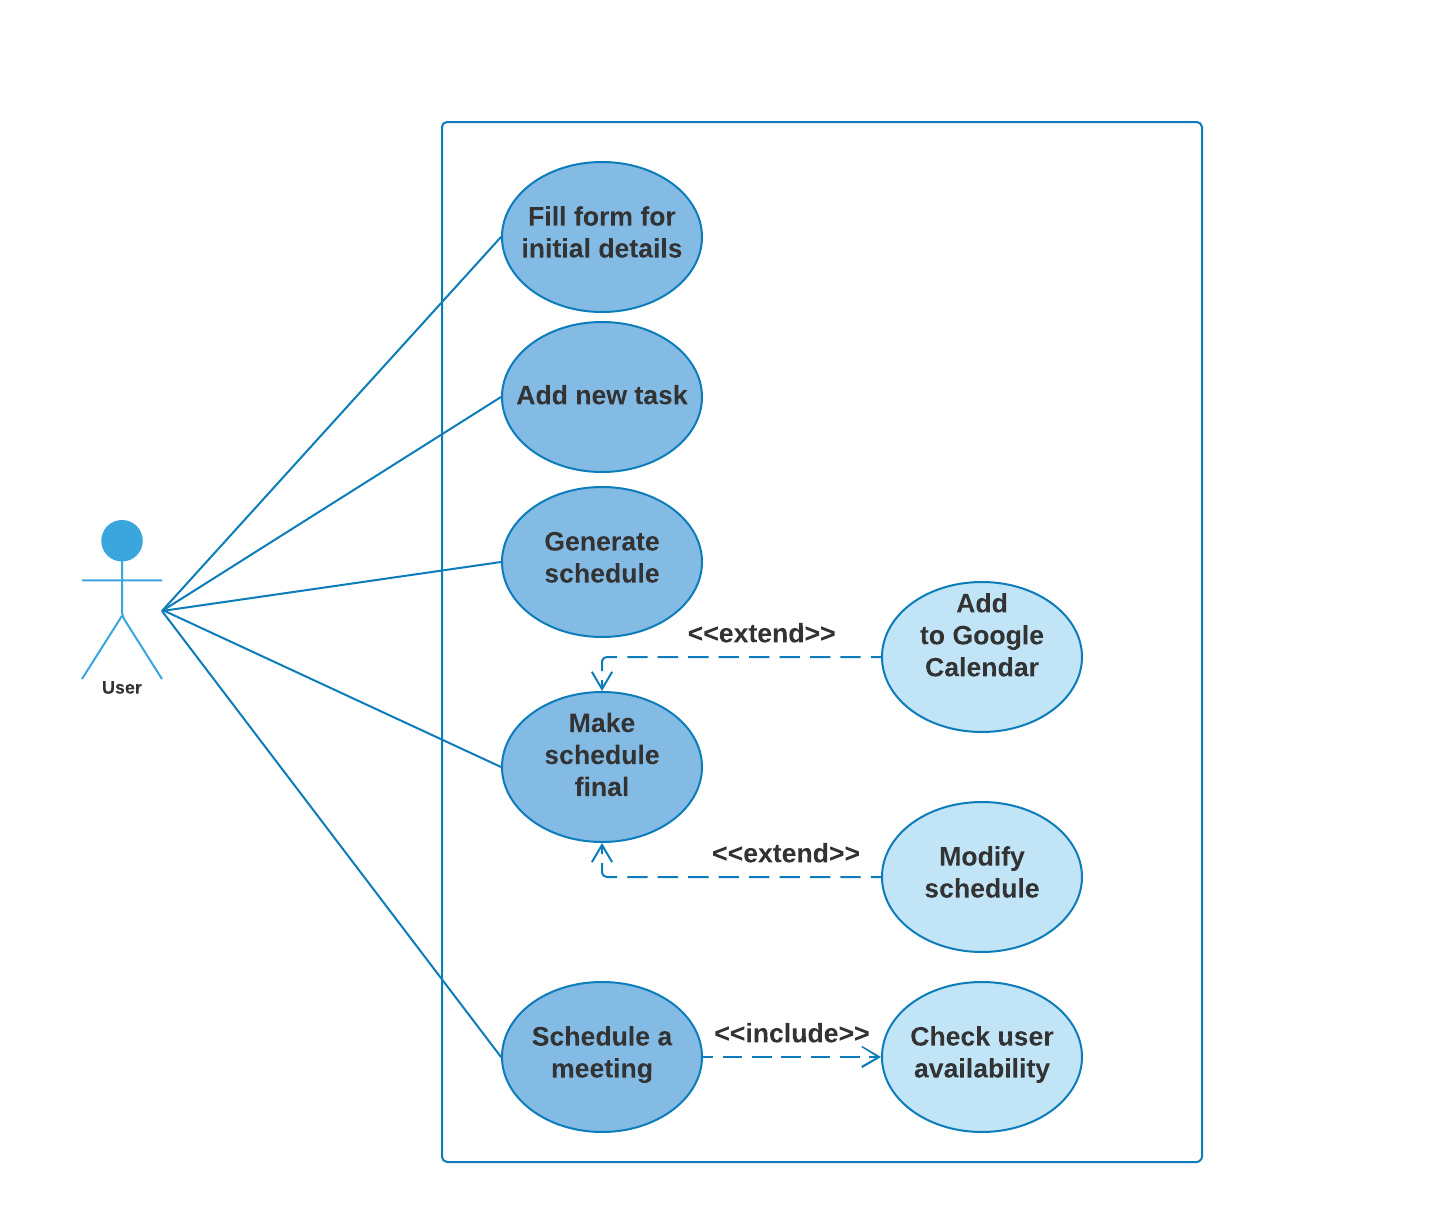
\includegraphics[scale = 0.32]{Use_Case_Diagram}
\centering
\caption{Use Case Diagram of the system}
% \vskip -6pt
\end{figure}
\FloatBarrier

\section{Survey}
We took a survey to find out how people are tackling issues of time management and whether they need such a product or not. The questions which we asked are as follows:
\begin{enumerate}
  \item \textbf{How often do you face difficulties in completing tasks because of not being able to manage time properly?}
  \par
  The purpose of this question was to understand if the people face difficulties in time management. 
  \par
  From the survey, the results tells us that there are not many people who do not experience the problem of task completion due to ineffective time management, so our bot might help to solve this problem.
\begin{figure}[!htbp]
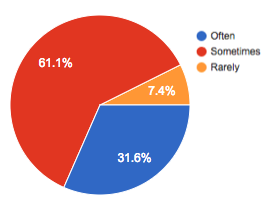
\includegraphics[scale = 0.5]{Difficulty}
\centering
\caption{Response for Question 1}
% \vskip -6pt
\end{figure}
  \item \textbf{Do you face an issue to set up project (or other) meetings due to conflicting schedules?}
  \par
  The purpose of this question so that we could evaluate the need of collaborative scheduling methods. 
  \par
  The results suggest that people do face the issue of setting up meetings as their schedules conflict. Hence, indicating a need of a collaborative personal scheduler.  
\begin{figure}[!htbp]
	
    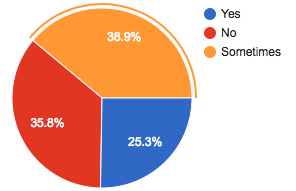
\includegraphics[scale = 0.5]{Meeting}
\centering
\caption{Response for Question 2}
\end{figure}
  \item \textbf{How much do you rely on Google Calendar (or similar) for planning your day-to-day tasks?}
  \par 
  This question was to understand the percentage of people depending on Calendar applications for daily use.
  \par
  This result tell us that people do not rely on calendar applications for planning their activities.But the following question (Q4) tells us that they do want a software which makes schedule for them.
    \begin{figure}[!htbp]
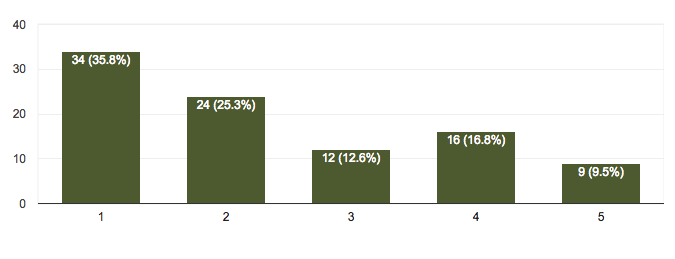
\includegraphics[scale = 0.3]{Calendar}
\centering
\caption{Response for Question 3}
% \vskip -6pt
\end{figure}
  \item \textbf{Do you feel the need for a software which makes a weekly schedule for you taking into account your pending tasks and preferences?}
  \par
  The results of this question showed us that more than three-fourth of the population need an application that helps the user. 
    \begin{figure}[!htbp]
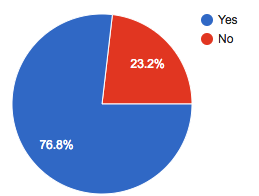
\includegraphics[scale = 0.5]{WantApp}
\centering
\caption{Response for Question 4}
% \vskip -6pt
\end{figure}
\end{enumerate}
\subsection*{Survey Conclusion}
\par
Based on the 92 responses we got from our survey we can conclude that a personalized time management bot will be very helpful for the people. Most of the respondents do face a problem of completing tasks efficiently due to lack of proper time management. Using a bot which will schedule tasks for the individual will help with proper management of tasks and also save the user's time as there is no need to schedule tasks manually. The bot will also take care of meeting scheduling which is hassle for some of the respondents. The survey tells us that not many people rely on calendar applications like Google Calendar for task scheduling but would like to use a software like our bot. From this result we can conclude that people will start using softwares similar to calendar applications for task scheduling if there are more important features like dynamic schedule generation . 


\section{Technologies}
\begin{enumerate}
  \item \textbf{MongoDB on AWS: } 
  We plan to use MongoDB\cite{planner5} Amazon Web Services'Database\cite{planner6} for storing user details and their tasks as individual objects.
  \item \textbf{Dialogflow: } 
  We plan to use Dialogflow\cite{planner7} for natural language processing in the implementation of the chatbot.
  \item \textbf{Slack: } 
  The platform for deploying the chatbot. We can integrate dialogflow with Slack\cite{planner8}.
  \item \textbf{Python: } 
  We will use this language for implementing our scheduling algorithm, for the API calls (Google Calendar and Dialogflow) and for establishing connection with AWS MongoDB Database.
  \item \textbf{Google Calendar API: } 
  We plan to use this API to provide an option to the users for adding their schedule to a widely used calendar service for easy integration between users.
\end{enumerate}

\section{Time-line}
\begin{enumerate}
\item \textbf{January 16th} - Read research papers in search of a topic.

\item \textbf{January 19th} - Shortlisted and eventually finalized a topic.

\item \textbf{January 21st} - Detailed problem definition developed, modules defined.

\item \textbf{January 23rd} - Technologies decided, researched scheduling algorithms. 

\item \textbf{January 26th} - Finalized the scheduling algorithm 

\item \textbf{January 28th} - Divided the tasks and started working on the modules.

\item \textbf{January 30th} - Made a demo bot using DialogFlow and designed schema for the database.

\item \textbf{February 1st} - Establishing connection between the bot and MongoDB database, setup the bot and start learning it.

\item \textbf{February 3rd} - Retrieval of data from database as input to the scheduling algorithm.

\item \textbf{February 6th} - Finish learning the bot for our basic model.

\item \textbf{February 10th} - Deployment of basic model which includes primary features like scheduling the tasks given by user. Also, we plan to start testing it after this.

\item \textbf{February 13th} - Start working on the application for additional functionalities suggested in tests or ones previously planned, like meeting scheduling.

\item \textbf{February 17th} - Start training the bot for additional functionalities.

\item \textbf{February 20th} - Start working on the first set of reviews given by users involved in beta testing.

\item \textbf{February 26th} - Complete training the bot which includes all the functionalities.

\item \textbf{February 28th} - Creating test cases for the final testing phase.

\item \textbf{March 7th} - Getting feedback from testing phase. Checking for bugs and thinking about approach and starting to fix the bugs.

\item \textbf{March 10th} - Finalizing the application with the fixes required.
\end{enumerate}


\section{Evaluation Plan}
As mentioned in the time-line, we intend to deploy a basic prototype by 10th February on Slack. Once deployed, we will test the prototype using Beta testing. We will collect inputs from the testers via Google form which will be prompted at the end. We plan to get our system evaluated by 30-40 testers in the Beta testing phase. 
\par
On receiving adequate feedback, we will work on the issues and/or improvements suggested. Also, we have a few functionalities which we plan to add if time permits. Once bug fixing and implementation of additional functionalities is done, we plan to deploy the fully functional prototype for use by the end of the month.
\begin{figure}[!htbp]
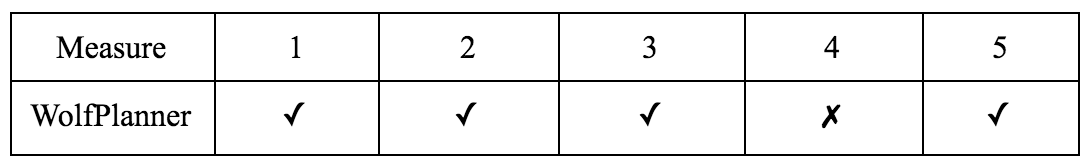
\includegraphics[scale = 0.4]{EP}
\centering
\caption{Evaluation Plan}
% \vskip -6pt
\end{figure}
\begin{enumerate}
\item \textbf{Security} - Our system is safe from external threats because of AWS security norms.
\item \textbf{Scalability} - Our system is scalable because of the resources AWS provides.
\item \textbf{Privacy} - Our system ensures privacy of the user because it does not allow a user to access any other user's schedule/tasks without the other user's permission.
\item \textbf{Reliability} - Our system will not be reliable since no backup is maintained of the data. If the server goes down or due to some system error data is lost, there will be no way to recover the data.
\item \textbf{Ease of use} - Our system is easy to use because of the interactive and easy to understand bot interface.
\end{enumerate}
\section{Future Scope}

\begin{enumerate}
\item \textbf{Integrating with the University Portal}
\par
Using the University portal, will save the students' time and effort. As the user will not have to enter details such as Courses, Exams and Assignment schedules. By integrating the application with the Portal will enable the Bot to fetch all of these details automatically. 
\item \textbf{Using Machine Learning for better customization}
\par
By applying machine learning techniques, the bot could learn to adjust the time slice assigned for a particular task based on past experience. This could be obtained by learning the time taken by the user to perform a similar task previously.

\item \textbf{Creating a new user: Professor/TA}
\par
We can create a new user type, Professor/TA who will decide and set time needed to complete certain tasks like assignments. This will be reflected automatically in the corresponding student users' schedule.

\end{enumerate}

\section{Conclusions}
The chatbot will generate a schedule for the student taking into account their deadlines and dependencies between their tasks. Our scheduling algorithm will take into consideration all the details such as classes, assignments, project meetings, discussions, readings, etc of the student. The chatbot will help the user focus on important tasks by automating the scheduling. Furthermore, the chatbot will also assist in collaborative meet-ups as per the user's request. Therefore, helping users in a team to communicate well. 
At the same time, the bot also makes it easier to access the generated schedule by providing an option to export to Google Calendar.

 
\begin{thebibliography}{999}

\bibitem{planner1}
  Gartner.com,
  \emph{ Gartner Customer 360 Summit 2011.} [Online].
  Retrieved from: \url{http://www.gartner.com/imagesrv/summits/docs/na/customer-360/C360_2011_brochure_FINAL.pdf} [Accessed: 23-Jan-2018].
  
\bibitem{planner2}
  Berry, Pauline, et al.
  \emph{ Deploying a personalized time management agent.}
  Proceedings of the fifth international joint conference on Autonomous agents and multiagent systems. ACM, 2006.

\bibitem{planner3}
  Schwiegelshohn, Uwe, and Ramin Yahyapour.
  \emph{Analysis of first-come-first-serve parallel job scheduling.}
SODA. Vol. 98. 1998
  
\bibitem{planner4}
Wilkerson, L. J., and J. D. Irwin.
  \emph{An improved method for scheduling independent tasks.}
  AIIE transactions 3.3 (1971): 239-245.

\bibitem{planner5}
MongoDB Documentation,
Retrieved from: \url{https://docs.mongodb.com/}
[Accessed:26-Jan-2018]
\bibitem{planner6}
  Amazon Web Services,
  \emph{MongoDB on AWS} April 2016
  Retrieved from: \url{https://d0.awsstatic.com/whitepapers/AWS_NoSQL_MongoDB.pdf
} [Accessed: 26-Jan-2018]
  \bibitem{planner7}
   Dialogflow,
  \emph{Dialogflow Reference Documentation}
  Retrieved from: \url{https://dialogflow.com/docs/reference/agent/}[Accessed: 26-Jan-2018]
   \bibitem{planner8}
   Slack,
  \emph{Getting started with the Slack API}
  Retrieved from: \url{https://api.slack.com/getting-started}[Accessed: 26-Jan-2018]


\end{thebibliography}

\end{document}
